% Options for packages loaded elsewhere
\PassOptionsToPackage{unicode}{hyperref}
\PassOptionsToPackage{hyphens}{url}
%
\documentclass[
  english,
  ,apa7,floatsintext]{apa6}
\usepackage{amsmath,amssymb}
\usepackage{lmodern}
\usepackage{ifxetex,ifluatex}
\ifnum 0\ifxetex 1\fi\ifluatex 1\fi=0 % if pdftex
  \usepackage[T1]{fontenc}
  \usepackage[utf8]{inputenc}
  \usepackage{textcomp} % provide euro and other symbols
\else % if luatex or xetex
  \usepackage{unicode-math}
  \defaultfontfeatures{Scale=MatchLowercase}
  \defaultfontfeatures[\rmfamily]{Ligatures=TeX,Scale=1}
\fi
% Use upquote if available, for straight quotes in verbatim environments
\IfFileExists{upquote.sty}{\usepackage{upquote}}{}
\IfFileExists{microtype.sty}{% use microtype if available
  \usepackage[]{microtype}
  \UseMicrotypeSet[protrusion]{basicmath} % disable protrusion for tt fonts
}{}
\makeatletter
\@ifundefined{KOMAClassName}{% if non-KOMA class
  \IfFileExists{parskip.sty}{%
    \usepackage{parskip}
  }{% else
    \setlength{\parindent}{0pt}
    \setlength{\parskip}{6pt plus 2pt minus 1pt}}
}{% if KOMA class
  \KOMAoptions{parskip=half}}
\makeatother
\usepackage{xcolor}
\IfFileExists{xurl.sty}{\usepackage{xurl}}{} % add URL line breaks if available
\IfFileExists{bookmark.sty}{\usepackage{bookmark}}{\usepackage{hyperref}}
\hypersetup{
  pdftitle={The Development of Color Terms in Shipibo-Konibo Children},
  pdfauthor={Martin Fortier*1, Danielle Kellier*2, María Fernández Flecha3, \& Michael C. Frank4},
  pdflang={en-EN},
  pdfkeywords={Shipibo-Konibo; Color; Word learning; Bilingualism},
  hidelinks,
  pdfcreator={LaTeX via pandoc}}
\urlstyle{same} % disable monospaced font for URLs
\usepackage{graphicx}
\makeatletter
\def\maxwidth{\ifdim\Gin@nat@width>\linewidth\linewidth\else\Gin@nat@width\fi}
\def\maxheight{\ifdim\Gin@nat@height>\textheight\textheight\else\Gin@nat@height\fi}
\makeatother
% Scale images if necessary, so that they will not overflow the page
% margins by default, and it is still possible to overwrite the defaults
% using explicit options in \includegraphics[width, height, ...]{}
\setkeys{Gin}{width=\maxwidth,height=\maxheight,keepaspectratio}
% Set default figure placement to htbp
\makeatletter
\def\fps@figure{htbp}
\makeatother
\setlength{\emergencystretch}{3em} % prevent overfull lines
\providecommand{\tightlist}{%
  \setlength{\itemsep}{0pt}\setlength{\parskip}{0pt}}
\setcounter{secnumdepth}{-\maxdimen} % remove section numbering
% Make \paragraph and \subparagraph free-standing
\ifx\paragraph\undefined\else
  \let\oldparagraph\paragraph
  \renewcommand{\paragraph}[1]{\oldparagraph{#1}\mbox{}}
\fi
\ifx\subparagraph\undefined\else
  \let\oldsubparagraph\subparagraph
  \renewcommand{\subparagraph}[1]{\oldsubparagraph{#1}\mbox{}}
\fi
% Manuscript styling
\usepackage{upgreek}
\captionsetup{font=singlespacing,justification=justified}

% Table formatting
\usepackage{longtable}
\usepackage{lscape}
% \usepackage[counterclockwise]{rotating}   % Landscape page setup for large tables
\usepackage{multirow}		% Table styling
\usepackage{tabularx}		% Control Column width
\usepackage[flushleft]{threeparttable}	% Allows for three part tables with a specified notes section
\usepackage{threeparttablex}            % Lets threeparttable work with longtable

% Create new environments so endfloat can handle them
% \newenvironment{ltable}
%   {\begin{landscape}\begin{center}\begin{threeparttable}}
%   {\end{threeparttable}\end{center}\end{landscape}}
\newenvironment{lltable}{\begin{landscape}\begin{center}\begin{ThreePartTable}}{\end{ThreePartTable}\end{center}\end{landscape}}

% Enables adjusting longtable caption width to table width
% Solution found at http://golatex.de/longtable-mit-caption-so-breit-wie-die-tabelle-t15767.html
\makeatletter
\newcommand\LastLTentrywidth{1em}
\newlength\longtablewidth
\setlength{\longtablewidth}{1in}
\newcommand{\getlongtablewidth}{\begingroup \ifcsname LT@\roman{LT@tables}\endcsname \global\longtablewidth=0pt \renewcommand{\LT@entry}[2]{\global\advance\longtablewidth by ##2\relax\gdef\LastLTentrywidth{##2}}\@nameuse{LT@\roman{LT@tables}} \fi \endgroup}

% \setlength{\parindent}{0.5in}
% \setlength{\parskip}{0pt plus 0pt minus 0pt}

% Overwrite redefinition of paragraph and subparagraph by the default LaTeX template
% See https://github.com/crsh/papaja/issues/292
\makeatletter
\renewcommand{\paragraph}{\@startsection{paragraph}{4}{\parindent}%
  {0\baselineskip \@plus 0.2ex \@minus 0.2ex}%
  {-1em}%
  {\normalfont\normalsize\bfseries\itshape\typesectitle}}

\renewcommand{\subparagraph}[1]{\@startsection{subparagraph}{5}{1em}%
  {0\baselineskip \@plus 0.2ex \@minus 0.2ex}%
  {-\z@\relax}%
  {\normalfont\normalsize\itshape\hspace{\parindent}{#1}\textit{\addperi}}{\relax}}
\makeatother

% \usepackage{etoolbox}
\makeatletter
\patchcmd{\HyOrg@maketitle}
  {\section{\normalfont\normalsize\abstractname}}
  {\section*{\normalfont\normalsize\abstractname}}
  {}{\typeout{Failed to patch abstract.}}
\patchcmd{\HyOrg@maketitle}
  {\section{\protect\normalfont{\@title}}}
  {\section*{\protect\normalfont{\@title}}}
  {}{\typeout{Failed to patch title.}}
\makeatother
\shorttitle{Color Terms in Shipibo-Konibo Children}
\keywords{Shipibo-Konibo; Color; Word learning; Bilingualism\newline\indent Word count: 9156}
\usepackage{lineno}

\linenumbers
\usepackage{csquotes}
\ifxetex
  % Load polyglossia as late as possible: uses bidi with RTL langages (e.g. Hebrew, Arabic)
  \usepackage{polyglossia}
  \setmainlanguage[]{english}
\else
  \usepackage[main=english]{babel}
% get rid of language-specific shorthands (see #6817):
\let\LanguageShortHands\languageshorthands
\def\languageshorthands#1{}
\fi
\ifluatex
  \usepackage{selnolig}  % disable illegal ligatures
\fi
\newlength{\cslhangindent}
\setlength{\cslhangindent}{1.5em}
\newlength{\csllabelwidth}
\setlength{\csllabelwidth}{3em}
\newenvironment{CSLReferences}[2] % #1 hanging-ident, #2 entry spacing
 {% don't indent paragraphs
  \setlength{\parindent}{0pt}
  % turn on hanging indent if param 1 is 1
  \ifodd #1 \everypar{\setlength{\hangindent}{\cslhangindent}}\ignorespaces\fi
  % set entry spacing
  \ifnum #2 > 0
  \setlength{\parskip}{#2\baselineskip}
  \fi
 }%
 {}
\usepackage{calc}
\newcommand{\CSLBlock}[1]{#1\hfill\break}
\newcommand{\CSLLeftMargin}[1]{\parbox[t]{\csllabelwidth}{#1}}
\newcommand{\CSLRightInline}[1]{\parbox[t]{\linewidth - \csllabelwidth}{#1}\break}
\newcommand{\CSLIndent}[1]{\hspace{\cslhangindent}#1}

\title{The Development of Color Terms in Shipibo-Konibo Children}
\author{Martin Fortier*\textsuperscript{1}, Danielle Kellier*\textsuperscript{2}, María Fernández Flecha\textsuperscript{3}, \& Michael C. Frank\textsuperscript{4}}
\date{}


\authornote{

Correspondence concerning this article should be addressed to Danielle Kellier*, Postal address. E-mail: \href{mailto:danielle.kellier@pennmedicine.upenn.edu}{\nolinkurl{danielle.kellier@pennmedicine.upenn.edu}}

}

\affiliation{\vspace{0.5cm}\textsuperscript{1} PSL Research University\\\textsuperscript{2} University of Pennsylvania\\\textsuperscript{3} Pontificia Universidad Católica del Perú\\\textsuperscript{4} Stanford University}

\abstract{
Color word learning is an important case study for the relationship between language and perception. While English color word learning is well-documented, there is relatively limited evidence on the developmental trajectory for color words, especially in languages from non-Western populations. We study color words and their acquisition in the Shipibo-Konibo (SK), an indigenous group within the Peruvian Amazon. In Study 1, we measure the color vocabulary in SK adults, updating findings from the World Color Survey. We then study receptive and productive knowledge of color words in children, conducted in both SK (Study 2) and Spanish (Study 3). Children learning the SK system show a protracted developmental trajectory towards adult-like color term knowledge compared to contemporary studies of English-speaking children. Further, when SK children lack precise color term knowledge, they appeared to follow different strategies for SK and Spanish, using Spanish vocabulary in SK and overgeneralizing in Spanish. For both children and adults, bilingual vocabulary is used adaptively to facilitate task performance, broadly supporting communicative views of color vocabulary.
}



\begin{document}
\maketitle

\hypertarget{introduction}{%
\section{Introduction}\label{introduction}}

Color is where language and perception meet. Words such as ``blue'' and ``red'' draw boundary lines across a perceptually continuous space of hues and shades. In English, there are 11 high frequency color terms that together span the color space, but this categorization system is not universal. For instance, Russian speakers use two distinct words to describe the colors light blue (``goluboy'') and dark blue (``siniy''); other languages have as few as two words {[}e.g., the Jalé people only have terms for ``light'' and ``dark''; Berlin and Kay (1969){]}. Why do languages vary in their color systems? One emerging consensus is that languages categorize the color spectrum in different ways in part due to functional demands (Gibson et al., 2017): both smaller and larger color systems are relatively optimal for different communicative needs (Regier et al., 2007; Zaslavsky et al., 2018).

Learnability is hypothesized to be one contributor to this cross-linguistic diversity (Chater \& Christiansen, 2010; Culbertson et al., 2012). Some color systems may be easier for children to learn than others, or children may show inductive biases that shape the color vocabulary. But the actual acquisition of color terms -- while relatively well-studied in English (e.g., Forbes \& Plunkett, 2019; Saji et al., 2015; Sandhofer \& Smith, 1999; Wagner et al., 2013, 2018) -- is relatively under-studied across other populations (cf. Forbes \& Plunkett, 2020).

In the current project, our goals were (1) to characterize color term knowledge in an indigenous population, the Shipibo-Konibo (SK), and then (2) to build on this foundation to characterize the developmental trajectory of color language acquisition in a group of children raised learning Shipibo-Konibo, a departure from the WEIRD (Western Educated Industrialized Rich Democratic) populations that are over-represented in behavioral science (Henrich et al., 2010; Nielsen et al., 2017). This work provides a developmental comparison to understand both consistencies and variabilities in the trajectory of color word learning for children who are growing up in environments with far fewer manufactured, multi-colored plastic toys (Gibson et al., 2017).

In the remainder of the introduction, we review color vocabulary development in children, and then we turn to what is currently known about color terms in Latin American varieties of Spanish, such as Mexican, Colombian, and Bolivian Spanish, and in some Amazonian languages, such as Candoshi, Pirahã, and Shipibo-Konibo. These two literatures set the stage for our own study.

\hypertarget{the-development-of-color-vocabulary}{%
\subsection{The Development of Color Vocabulary}\label{the-development-of-color-vocabulary}}

To adults, colors are extremely salient attributes of the perceptual world; even when color is seemingly task-irrelevant, we mention it (e.g., Sedivy, 2003). It is quite surprising then that children sometimes struggle to master color vocabulary. Early observations by Darwin, Bateman, Nagel, and others attest to individual children's delays in the correct use of color terms well into middle childhood; several diarists report 5- to 8-year-olds with limited mastery of basic level color terms (reviewed in Bornstein, 1985). These observations are surprising in light of the body of infant research that suggests that infants' color discrimination abilities are relatively well-developed by the end of the first year of life (for review see e.g., Bornstein, 2015).

Indeed, the age at which color words are learned has been shifting over the past hundred years, at least for English-speaking children. Bornstein (1985) documents substantial decreases in the age at which many children master their colors, citing four years as an age at which most children are proficient. In fact, this age may have even decreased further in the last thirty years, judging from recent studies (Forbes \& Plunkett, 2019; Wagner et al., 2013, 2018). What makes color words hard to learn, and why are they getting easier?

One prominent account of what makes color word learning difficult is that children may not recognize that color words pick out the perceptual dimension of hue at all (Bartlett, 1977; Sandhofer \& Smith, 1999), and that once they do, children rapidly map colors correctly onto the appropriate range of hues in color space. This account nicely explains the observation that there is often a period during which children will produce an inappropriate color word when asked ``what color is this?'' -- they know that color words go together and answer a particular question, they just don't know which color is which. A further point of parsimony for this account is that infants' color boundaries are not all that different in their placement from those of adults; thus, presumably the mapping task they face -- from words to hues -- is not all that difficult, once they recognize the dimension that they are attempting to map (Bornstein et al., 1976; Franklin et al., 2005).

On the other hand, when children's mapping errors are examined in detail, they show more systematicity than would be predicted by this account. Wagner et al. (2013) show that children who have not yet fully mastered the color lexicon nevertheless use colors in ways that are more consistent with overextension than with ignorance of the dimensional mapping -- for example, using ``blue'' to refer to \emph{blue} and \emph{green} hues (which are close together in color space). These overextensions are reminiscent of noun overextensions that have been documented in early word learning, for example calling a horse ``dog'' (Clark, 1973). Further, the order of acquisition for color word meanings in Wagner et al. (2013) was well-predicted by the frequency and perceptual salience of color categories (Yurovsky et al., 2015), supporting the view that color categories are learned gradually from perceptual experiences rather than all at once. Finally, both behavioral and eye-tracking evidence suggest that children show earlier comprehension than production for color words (Forbes \& Plunkett, 2019; Sandhofer \& Smith, 1999; Wagner et al., 2018), a phenomenon that is seen throughout early word learning. In eye-tracking tasks, comprehension also shows evidence of perceptual overextensions, such that children fixate perceptually close distractor colors more than far distractors (Wagner et al., 2018). In sum, although attention to the dimension of hue may be one difficult component of color word learning, systematic mapping of words to particular regions of perceptual space is likely another.

Why is color word learning occurring earlier in development, at least for English-learning children (Bornstein, 1985)? There are at least two obvious, plausible reasons. The first is the increasing prevalence of manufactured toys for children that vary exclusively in color (e.g., sets of plastic blocks of different colors) (Gibson et al., 2017). Such objects provide perfect contrastive input for mapping: if one is called ``blue'' and the other is not, such input implicates pragmatically that ``blue'' is an informative term (Clark, 1987; Frank \& Goodman, 2014). The second is a cultural landscape for parents and early educators that presupposes color words are an important part of early childhood education practices, and as such should be taught explicitly (perhaps using toys specifically made for this purpose).

In the current paper, we ask about the trajectory of color word learning in an environment where both factors are less prevalent: that is, manufactured toys are less frequent, and parents are (at least anecdotally) less motivated to provide color labels to their children. Here we are inspired by the work of Piantadosi et al. (2014), who studied the learning of number word meanings in children in an Amazonian culture. They found that, despite differences in developmental timing, the patterns of generalization of number meaning were generally similar to those documented in WEIRD populations. We are interested in whether we observe similar dynamics in color word learning. In the next section, we turn to the question of adults' color vocabulary in Spanish and Amazonian language, setting the stage for our studies of acquisition.

\hypertarget{color-in-latin-american-varieties-of-spanish-and-amazonian-languages}{%
\subsection{Color in Latin American varieties of Spanish and Amazonian languages}\label{color-in-latin-american-varieties-of-spanish-and-amazonian-languages}}

Since the color systems local to the SK provide a backdrop for our work, in this section, we provide a brief overview of descriptive work on Latin American Spanish and some Amazonian languages. In brief, our conclusion is that ad hoc color terms -- descriptors of objects or properties that are adopted for the description of hue (e.g., the use of terms like ``blood'' or ``bloody'' to refer to red objects) -- are quite common, presaging some of our findings. They are likey present in several Latin American Spanish dialects and they are well-attested in Amazonian color systems.

An initial framework for the cross-linguistic study of color came from the World Color Survey {[}WCS; Kay et al. (2009){]}. WCS presented adult speakers of over 100 languages with differently colored chips and asked them to produce a label, characterizing the space of color vocabulary in a range of written and unwritten languages. The WCS focused on basic level color terms, the color words that are highest frequency and most consistently used.

The WCS framework has been revised and questioned in subsequent work, however (e.g., Levinson, 2000). In particular, there has been significant controversy about the applicability of the framework to Amazonian languages, centered around the status of ad hoc color terms. Such ad hoc terms are a common way that languages supplement color vocabulary (e.g., Kristol, 1980). Historical case studies suggest that ad hoc terms can often become conventionalized basic level color terms {[}e.g., the English color ``orange'' derives from an ad hoc term based on the fruit; St. Clair (2016){]}.

Since the WCS, however, later research has suggested that ad hoc terms are present in some South American dialects of Spanish and that they play a central role in Amazonian color systems. With respect to Spanish, the WCS identified the following basic level terms in the Mexican dialect: ``blanco'' (white), ``negro'' (black), ``rojo'' (red), ``verde'' (green), ``amarillo'' (yellow), ``azul'' (blue), ``café'' (brown or coffee-colored), ``morado'' (purple), ``rosa'' (pink or rose), ``anaranjado'' (orange, strictly referring to the color) and ``gris'' (gray). However, Aragón (2016) offers an ethnolinguistic study of color terms in Mexican Spanish and concludes that the local natural and cultural referents constitute a point of consensus among Mexicans when defining terms of color, even though these colors still follow the general schema of basic level terms. Further, Monroy and Custodio (1989) suggest that Columbian Spanish may include ad hoc color terms referring to colors through objects prototypically instantiating these colors (e.g., vegetables, animals, food, metals, precious stones, fire and its derivatives, and atmospheric phenomena). Lillo et al. (2018) generally confirm these observations, finding an additional basic level term in Uruguayan Spanish, ``celeste'' (sky blue), which may be a conventionalized ad hoc term (``celeste'' is etymologically related to ``sky''). This observation is also confirmed by Gibson et al. (2017) for Bolivian Spanish.

Turning now to Amazonian languages, SK color terms were studied in the original WCS. In this data collection effort, they list 21 distinct terms (though this could be categorized as 20 as ``huiso'' and ``wiso'' are alternative spellings of the same color term).\footnote{Two anthropological studies (Morin, 1973; Tournon, 2002) have also investigated the color terms used in SK. However, these two studies contain some serious methodological pitfalls: a very limited number of color chips were tested with only a few participants. As a result, we will not further discuss these studies in the remainder of this article and will only focus in our study on a comparison with the WCS data.} As their protocol has the field experimenters ask only for basic level color terms, it is assumed that all recorded terms are basic, but only six terms appear in \textgreater5\% of WCS trials; 10 terms appear in \textless1\% of trials (see Figure \ref{fig:study1-figure}A for a representation of this data). Immediately the issue of ad hoc terms rears its head, since it is likely that many of these other words are ad hoc color terms (Levinson, 2000).\footnote{In fact, a greater diversity of color terms beyond the basic level is used in the data for the majority of WCS languages (Gibson et al., 2017, Figure S1), suggesting that the effort to elicit only basic level color terms in WCS may not have been successful.}

Several other indigenous Amazonian color systems were studied in the WCS and one of them, Candoshi, has been examined more recently (Surrallés, 2016). Contrary to the WCS, Surrallés argues that no proper color terms exist in this language. If the fieldworkers of the WCS found otherwise, he claims, it is only because they misidentified the elicited terms as basic level color terms when they are nothing more than a series of ad hoc terms referring to objects or animals of the surrounding environment. For example, in Candoshi, the word for yellow is ``ptsiyaromashi'' (``like the feathers of a milvago bird''), the word for red is ``chobiapi'' (``ripe fruit''), the word for green is ``kamachpa'' (``unripe fruit''), etc. These findings lead Surrallés to argue that the Candoshi do not have a proper color system. When they use ``color terms'' they are not trying to subsume objects of the world under abstract color categories, but they are rather establishing horizontal and ad hoc comparisons between similar objects of the world.

A similar criticism of the WCS approach was given by Everett (2005) based on his study of Pirahã, another Amazonian language. Everett also rejected the idea that there are basic level terms, arguing that the four color terms identified as basic in the WCS are not such. For example, the word identified as the basic level for \emph{red}/\emph{yellow} in Pirahã (``bi i sai'') was argued to be simply a property descriptor meaning ``blood-like.'' The argument here is that Pirahã color terms might be ad hoc comparisons rather than proper basic terms, though there was no quantitative evaluation of this claim such as analysis of the variability in term use.

Finally, Gibson et al. (2017) compared their Bolivian Spanish data with Tsimane, a language of the Amazonian piedmont. Out of a total of 80 color chips, the Tsimane system exhibited 8 apparently basic color terms. However, in their free-choice paradigm, Tsimane speakers showed high variability in nearly all the color terms used for all color chips presented in their study. Thus, Tsimane speakers appear to show substantial ad hoc term usage as well.

\hypertarget{the-current-study}{%
\subsection{The Current Study}\label{the-current-study}}

The Shipibo-Konibo people are an indigenous group located within the Peruvian Amazon. They are mainly horticulturalists, fishermen, occasionally hunters but are noted for their strong display of tradition (e.g.~via traditional art) despite increasingly regular interactions with the western world. They are also skilled traditional artists or artisans, resorting to these activities as a way to earn an income for their household. Their children receive formal schooling for 4 hours a day, both in SK\footnote{The phonemic inventory of SK language has 4 vowels (/i/, /ɨ/, /a/ and /o/) and 15 consonants: 3 plosives (/p/, /t/ and /k/), 2 affricates (/ts/ and /ʧ/), 2 nasals (/m/ and /n/), 5 fricatives (/β/, /s/, /ʃ/, /ʂ/, /ɦ/), and 3 approximants (/w/, /ɻ/ and /j/).} and Spanish. The amount of Spanish input they receive at school increases towards adolescence when they enter secondary education. There can be variation in how both languages coexist in the school setting from one village to another. Most SK adults are considered SK-Spanish bilinguals to different degrees although the elders may have only a minor grasp on Spanish.

The SK are an interesting group to examine from the perspective of color word learning. Although their cultural experience is quite different from the English-speaking WEIRD populations who have been the focus of color word acquisition studies, they are not an isolated hunter-gatherer group. Because of their location on the Ucayali River, one of the main tributaries of the Amazon, the SK culture has always been enmeshed in rich trading networks involving other indigenous groups of the Andes and the Lowlands (in pre-conquest times) as well as Mestizos and Westerners (in post-conquest times) (Lathrap, 1970). It would thus be mistaken to think of this culture as an ``isolated'' or ``preserved'' one. On the contrary, having been extensively exposed to numerous influences, the SK culture has been constantly reworked and reshaped through the centuries. The first deep transformation in Shipibo-Konibo culture can be traced to the 18th century, when Shipibos, Konibos and Shetebos were forced to live together by Franciscan evangelization (Myers, 1974). Later, the second half of the 20th century was characterized by intense contact with the Spanish-speaking Mestizo populations established along the Ucayali River. As a result, today's SK culture straddles two worlds: children grow up in a traditional culture but with some exposure to formal education and -- critically -- some of the manufactured, colored plastic goods that have been argued to create a need for rich color vocabulary (Gibson et al., 2017).\footnote{Access to manufactured goods varies across SK villages based in part on how close they are to Pucallpa, the regional capital.}

Further, the SK are heavily bilingual. To our knowledge, relatively little work has looked at effects of bilingualism on color word learning. Yet, with much of the world's population growing up multilingual, it is important to characterize how learners navigate a conceptual space where they may have words that appropriately name a target concept, but in a different language.

In Study 1, we examine the color vocabulary of current SK adults, comparing their vocabulary to results from the World Color Survey (a gap of more than 50 years). Next, we examine SK children's color vocabulary, focusing on their knowledge and their generalization of color terms across both SK (Study 2) and Spanish (Study 3). Through these three studies, we attempted to answer four primary research questions:

\begin{enumerate}
\def\labelenumi{\arabic{enumi}.}
\tightlist
\item
  What is the color vocabulary of SK and how has it changed since the WCS data collection effort?
\item
  What is the developmental timeline of color term acquisition in a non-WEIRD population that has fewer industrial products (toys) and less formal early childhood education?
\item
  Is the developmental course -- especially with respect to generalization and the dynamics of comprehension and production -- similar to that which has been documented in studies of English color term learning?
\item
  How is color term learning development affected by bilingual exposure in this group?
\end{enumerate}

To presage our conclusions, we find that SK color vocabulary has remained relatively consistent, with the exception of some intrusions from Spanish in areas of low coverage by the SK color system. Children learning the SK system show a protracted developmental trajectory towards adult-like knowledge compared with modern descriptive studies in WEIRD contexts. Further, when children lack precise color term knowledge, they appear to follow different strategies for SK and Spanish: for SK, children fell back on Spanish knowledge, while for Spanish, we observed substantial over-generalization of terms (Wagner et al., 2013, 2018). Finally, we find that children draw on their Spanish knowledge especially for colors where there is high uncertainty among adult speakers, suggesting that they are adaptively using their bilingual knowledge to facilitate accurate naming.

\hypertarget{study-1}{%
\section{Study 1}\label{study-1}}

Before we could assess the developmental trajectory of color term knowledge in SK children, our goal was to replicate and update the characterization of the adult SK color system given by the World Color Survey. As the WCS study took place generations prior, we could not assume the SK color term mappings had remained static, especially through years of industrialization and exposure to the Spanish language and its own color term system. As such, Study 1 used a modified version of the original WCS protocol, with an identical color chip set (subsampled to decrease task length). The goals were to characterize the current SK vocabulary and to generate a standard of adult knowledge against which subsequent child participants could be scored.

\hypertarget{methods}{%
\subsection{Methods}\label{methods}}

\hypertarget{participants}{%
\subsubsection{Participants}\label{participants}}

Our protocol for Study 1 and all subsequent studies received ethical approval from Pontificia Universidad Católica del Perú's Institutional Review Board. We recruited 39 adult participants (7 men). We experienced difficulty recruiting male participants as many of the men were away from the village during the day, resulting in a sample that was predominantly female. Most participants (31, 4 men) were from SK villages of the Middle Ucayali region (Yarinacocha, San Francisco, and Nueva Betania), with a subset from communities of the Lower (Paoyhan) and Upper (Puerto Belén) Ucayali regions. Within the small town of Yarinacocha (in the vicinity of Pucallpa), we recruited participants (9, 2 men) from Bena Jema, a predominantly SK neighborhood. All the other recruitment sites were native community villages with exclusively SK residents but a strong relationship with the outside world. Overall, the sample included SK adults who could be characterized as more urban (Yarinacocha and San Francisco sites) or more traditional and in regular contact with the surrounding rainforest (Nueva Betania, Paoyhan, and Puerto Belén sites).

The median age for participants was 38 years (\emph{IQR} = 26-48) ranging from 20 to 64 years. Regarding occupations, 41\% of the 32 female participants were homemakers or housewives (33\% of the overall sample) and another 41\% were artisans (33\%). Three of the 7 male participants (43\%, 8\% overall) were horticulturalists. Across both sexes, 5 women (16\%, 13\% overall) and 3 men (43\%, 8\% overall) identified as students, comprising a total of 21\% of the population. Although all adult participants were required to be native SK speakers, all were introduced to the Spanish language prior to adolescence (median age = 8yo, \emph{IQR} = 5-10).

\hypertarget{materials-and-procedure}{%
\subsubsection{Materials and procedure}\label{materials-and-procedure}}

Similar to the original WCS, we used a set of 330 Munsell color chips and asked participants to name them (Berlin \& Kay, 1969). We made a number of changes to the procedure, however. In the WCS, every participant provided terms for all 330 chips. Due to fear of participant fatigue, we split up color chips based on their ID numbers (even or odd) and participants were randomly assigned to work with either even- or odd-numbered color chips. As a result, each participant was presented with only 165 chips. All 330 hues within the set are visualized in Appendix 1. Dimensions of the chips were 2 cm × 2.5 cm.

First, the experimenter explained the general procedure and goals of the study to the participant. The experimenter would then present a single color chip to the participant and ask in SK: ``What is the color of this chip?'' The study was conducted solely in SK language with the assistance of a bilingual SK- and Spanish-speaking research assistant. It should be noted that although the experiment was conducted in SK, the SK word for color used is identical to the Spanish word \emph{color} (an example of SK speakers adopting Spanish words into their lexicon), which might have encouraged Spanish language use.

Besides the reduction in set size, our procedure also differed from that of WCS (see Kay et al., 2009, pp. 585--591) in other aspects. Participants sat in front of the experimenter. To manage changes in natural light intensity between participants, the experiment took place indoors near a window or a door instead of outdoors. Another difference between our study and the WCS procedure is in our approach for encouraging participants to describe chips using basic level color terms. In the WCS, the experimenter would instruct participants to only provide basic level color terms during the task (e.g., describing a chip as ``blue'' as opposed to ``navy blue'' or ``sky-like''). However, we had difficulties concisely explaining the concept of a basic level term compared to other terms.\footnote{Indeed, as Kay et al. (2009, pp. 587--589) acknowledge, there is no straightforward necessary and sufficient criteria for the basicness of a color term (cf Levinson, 2000).} We decided to allow participants to describe a chip with any term they wished, and to ask further questions to elicit a basic level term when they did not do so on their first try. For example, when presented with a red color chip, the participant might use the term ``blood-like'' (a non-basic term). The experimenter would then ask: ``Do you know of any other word to refer to the color of this chip?'' Should the participant subsequently respond with ``dark red'' (another non-basic level term), the experimenter would further ask: ``How would you refer to this color with only one word?'' Eventually, the participant might use the term ``red'' (a basic term). For some chips, participants provided a basic level term as their first description. For others, a basic level term might be preceded by 1 or 2 non-basic level terms. When participants failed to provide a basic level term after 3 attempts (i.e., two follow-up questions), no further questions were asked, and the experimenter moved on to the next chip. All responses, basic level or not, were recorded in the order produced by the participant.

\hypertarget{results-and-discussion}{%
\subsection{Results and Discussion}\label{results-and-discussion}}

Figure \ref{fig:study1-figure} compares the original WCS data (Panel A) to a summary of results (Panel B) along with the prevalence of Spanish-language responses (Panel C) for Study 1. All participants used the following set of color terms to describe a color chip at least once during their session: ``joxo'' (light/white), ``wiso'' (dark/black), ``panshin'' (yellow), ``joshin'' (red), and ``yankon'' (green/blue). Given the widespread use of this term set and their interpretations, we will refer to these five terms as SK-language basic level color terms

Most (79\%) participants also described at least 1 chip as ``manxan'' (faded), referring to a chip's saturation. In addition, fifty-one percent of participants used the color term ``naranja'' (or ``naransha'') to describe at least one chip. ``Naranja'' may be known as a Spanish-language color term used to describe both the orange fruit and its associated color--as opposed to ``anaranjado,'' a term strictly for the orange color.

In terms of overall popularity, participants described a median of 32\% of chips as ``yankon'' (\emph{IQR} = 26-39\%) followed by ``joshin'' (\emph{Mdn} = 10\%, \emph{IQR} = 7-16\%), ``panshin'' (10\%, 6-12\%), ``joxo'' (9\%, 6-15\%), ``manxan'' (6\%, 1-10\%), and ``wiso'' (5\%, 3-8\%). We failed to find any significant sex differences in the overall spread of color term usage across chip set (\(t(59) = 0.00\), \(p > .999\)) or in the proportion of subjects who used a term at least once during their session (\(t(117.95) = -0.38\), \(p = .706\)).

Compared to the WCS dataset which only reported SK language terms, Spanish use was prevalent throughout Study 1. Fifty-nine percent of our participants used a Spanish-language color term to describe at least 1 chip, which accounted for only 4\% of all responses. Across chips, the most common Spanish-language color term was ``naranja'' (51\% of participants), followed by ``rosa'' (10) and ``morado'' (8). Spanish use peaked at 55\% when participants were asked to label chips that English speakers would consider to be orange or ``anaranjado''/``naranja'' by Spanish speakers. Indeed, the relatively common use of ``naranja'' by these adult SK speakers despite being prompted entirely in SK brings the possibility that ``naranja'' has been adopted into the SK color lexicon. If we allow ``naranja'' to be counted as an SK rather than Spanish-language term, then only 15\% of participants used a Spanish-language term other than ``naranja'' at least once throughout the study, accounting for 2\% of all responses. One participant responded in Spanish in 68\% of the time despite being prompted solely in SK.

\begin{figure}
\centering
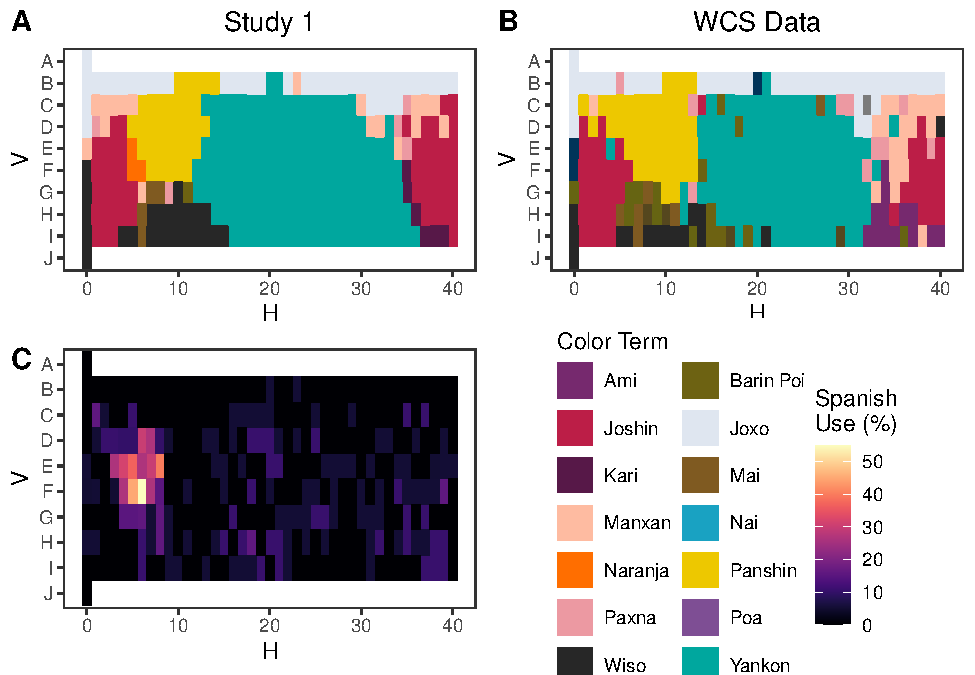
\includegraphics{amazon_color_files/figure-latex/study1-figure-1.pdf}
\caption{\label{fig:study1-figure}(A and B) Plots of the modal term given for a particular chip. Color coordinates were represented in 2-D Munsell space, with Munsell hue represented on the x-axis and Munsell value or lightness represented on the Y-axis. Modal responses were given by SK adults during (A) our Study 1 and during (B) the original World Color Survey. (C) Heat map of prevalence of Spanish-language responses during Study 1. Legends for all three subplots located in the bottom-right quadrant.}
\end{figure}

Participants used an SK-language basic level term (i.e., ``yankon'') to describe a median of 68\% of chips (\emph{IQR} = 56-90\%). Besides basic level terms, 59\% of participants used SK-language ad hoc color terms (i.e., ``nai'' or sky for blue chips) for an overall median of 6\% of chips (\emph{IQR} = 0-19\%). SK-language terms referring to saturation or luminosity of a chip, such as ``manxan'' (faded) were used for an overall median of 13\% of chips (\emph{IQR} = 6-20\%). Most instances (86\%) of Spanish use involved a Spanish BCT such as ``rojo'' (overall \emph{Mdn} = 0\%, \emph{IQR} = 0-0\%).

In sum, our data show similar variability to the WCS data, but with Spanish terms (as described above) mixed in with ad hoc terms. Notably, we observed the modal term for a few chips to be loanwords from Spanish, in some cases already established as part of the SK vocabulary (the last seems to be the case of ``naranja,'' ``orange'' in English), suggesting some fairly extensive borrowing of Spanish words due to the close relationship between both languages in the studied communities.

\hypertarget{study-2}{%
\section{Study 2}\label{study-2}}

After generating an updated SK color term map using the responses from adult participants in Study 1, we designed Study 2 to assess child participants' production and comprehension of SK color terms. Because we did not think that we could feasibly ask children across a range of ages about more than 100 color chips, we selected a subset of chips representing the prototypical instances for prominent SK terms from Study 1.

\begin{table}[tbp]

\begin{center}
\begin{threeparttable}

\caption{\label{tab:study23-demographics}Demographics of participants in Studies 2 and 3.}

\begin{tabular}{lll}
\toprule
Age Group & \multicolumn{1}{c}{n} & \multicolumn{1}{c}{Boys}\\
\midrule
\multicolumn{3}{c}{Study 2}\\
5 & 3 (5\% of overall sample) & 1\\
6 & 8 (14\%) & 3\\
7 & 12 (21\%) & 4\\
8 & 15 (26\%) & 5\\
9 & 10 (18\%) & 5\\
10 & 4 (7\%) & 2\\
11 & 5 (9\%) & 3\\
\multicolumn{3}{c}{Study 3}\\
5 & 2 (4\% of overall sample) & 1\\
6 & 2 (4\%) & 0\\
7 & 11 (24\%) & 4\\
8 & 9 (20\%) & 1\\
9 & 11 (24\%) & 4\\
10 & 8 (17\%) & 3\\
11 & 3 (7\%) & 3\\
\bottomrule
\end{tabular}

\end{threeparttable}
\end{center}

\end{table}

\hypertarget{methods-1}{%
\subsection{Methods}\label{methods-1}}

\hypertarget{participants-1}{%
\subsubsection{Participants}\label{participants-1}}

Fifty-seven children (23 boys) ages 5- to 11-years-old were recruited in predominantly SK neighborhoods in Yarinacocha (Nueva Era and Bena Jema) and in Bawanisho, a native community settled along the Ucayali River, more than 500 kilometers southeast of Pucallpa. Recruitment occurred either through direct contact with interested parents or through their local school. If recruited via school, consent for participation had to be given by both teacher and parent. Outside of the school environment, consent was given by the parent.

\hypertarget{materials-and-procedure-1}{%
\subsubsection{Materials and procedure}\label{materials-and-procedure-1}}

Based on the findings of Study 1, we chose 8 color chips from our original set of 330 to serve as prototypical instances of major SK color terms. These color chips were blue (WCS n°1), green (n°234), red (n°245), white (n°274), yellow (n°297), black (n°312), greenish-yellow (WCS n°320), and purple (WCS n°325). Study 2 was conducted entirely in SK and participants were explicitly instructed to give responses in SK as opposed to Spanish. In the production and comprehension tasks, children sat at a table across from the experimenter with color chips arranged between them. The production task was always performed before the comprehension task.

\hypertarget{production-task}{%
\subsubsection{Production task}\label{production-task}}

Similar to Study 1, the experimenter introduced the participant to the general procedure and the goals of the study. The experimenter would then ask: ``What is the color of this chip?'' As in Study 1, we used follow-up questions to elicit a basic level term when the child's initial response was not one. In a departure from Study 1, we were more explicit in soliciting an SK-language response. When a participant provided a Spanish-language term, the experimenter would record their response but further ask: ``What is the name of this color in SK?'' If a participant could not respond with an SK term, the experimenter would not ask further questions and would move forward to the next chip. As a result, some children only produced SK non-basic level terms or Spanish-language terms for particular chips.

\hypertarget{comprehension-task}{%
\subsubsection{Comprehension task}\label{comprehension-task}}

The comprehension task had a notably different procedure compared to the preceding production task. We tested the comprehension of 9 SK color terms. The choice of these terms was based on common responses given by adult participants in Study 1. The color term prompts included basic level terms: ``yankon'' (green/blue), ``joshin'' (red), ``panshin'' (yellow), ``joxo'' (white/light), ``wiso'' (black/dark). We also included non-basic but prominent terms as prompts which were ``nai'' (sky or sky blue), and ``barin poi'' (greenish-yellow, meaning the Sun´s excrement, also used to refer to an alga) and two dyads of non-basic terms: ``pei'' (leaf) and ``xo'' (unripe) to represent the color green, along with ``ami'' (a type of tree used to dye fabrics) and ``pua'' (sachapapa, a tuber) to represent purple. Children sat at a table across from the experimenter with the 8 color chips of the production task displayed between them. The experimenter asked: ``Can you give me the {[}\emph{color term}{]} chip?'' Participants chose one of the 8 chips and their response was recorded.

Our findings from Study 1 suggested that color terms varied in their degrees of specificity. For example, ``wiso'' best describes a narrow range of very dark to black. By contrast, ``yankon'' could encompass blue, green, greenish-yellow, and purple; ``joshin'' could describe red, purple, and orange; ``pei'' or ``xo'' could describe green or greenish-yellow. In cases where a term could apply to multiple chips (i.e., ``yankon''), the chip selected first would be removed from the table, leaving 7 remaining chips. The experimenter would then ask: ``Can you give me another {[}\emph{color term}{]} chip?'' The participant would then pick another one of the 7 chips, have their response recorded, and so on. We prompted participants 4 times for ``yankon'' and 2 times each for ``joshin'' and ``pei''/``xo''; every other term only received a single prompt. Due to the inherent ambiguity in term-hue pairings, accuracy for a child participant was coded based on adult responses given during Study 1. If at least 15\% of adult participants in Study 1 associated a chip with a particular term, we coded a similar term-chip pairing from a child participant as correct. Some trials could have multiple pairings; in those cases, accuracy was scored as an average, rather than as dichotomous. For instance, if a child correctly chose 3 out of 4 chips for the ``yankon'' trial, instead of 1 (correct) or 0 (incorrect) they would receive a score of 0.75.

\begin{figure}
\centering
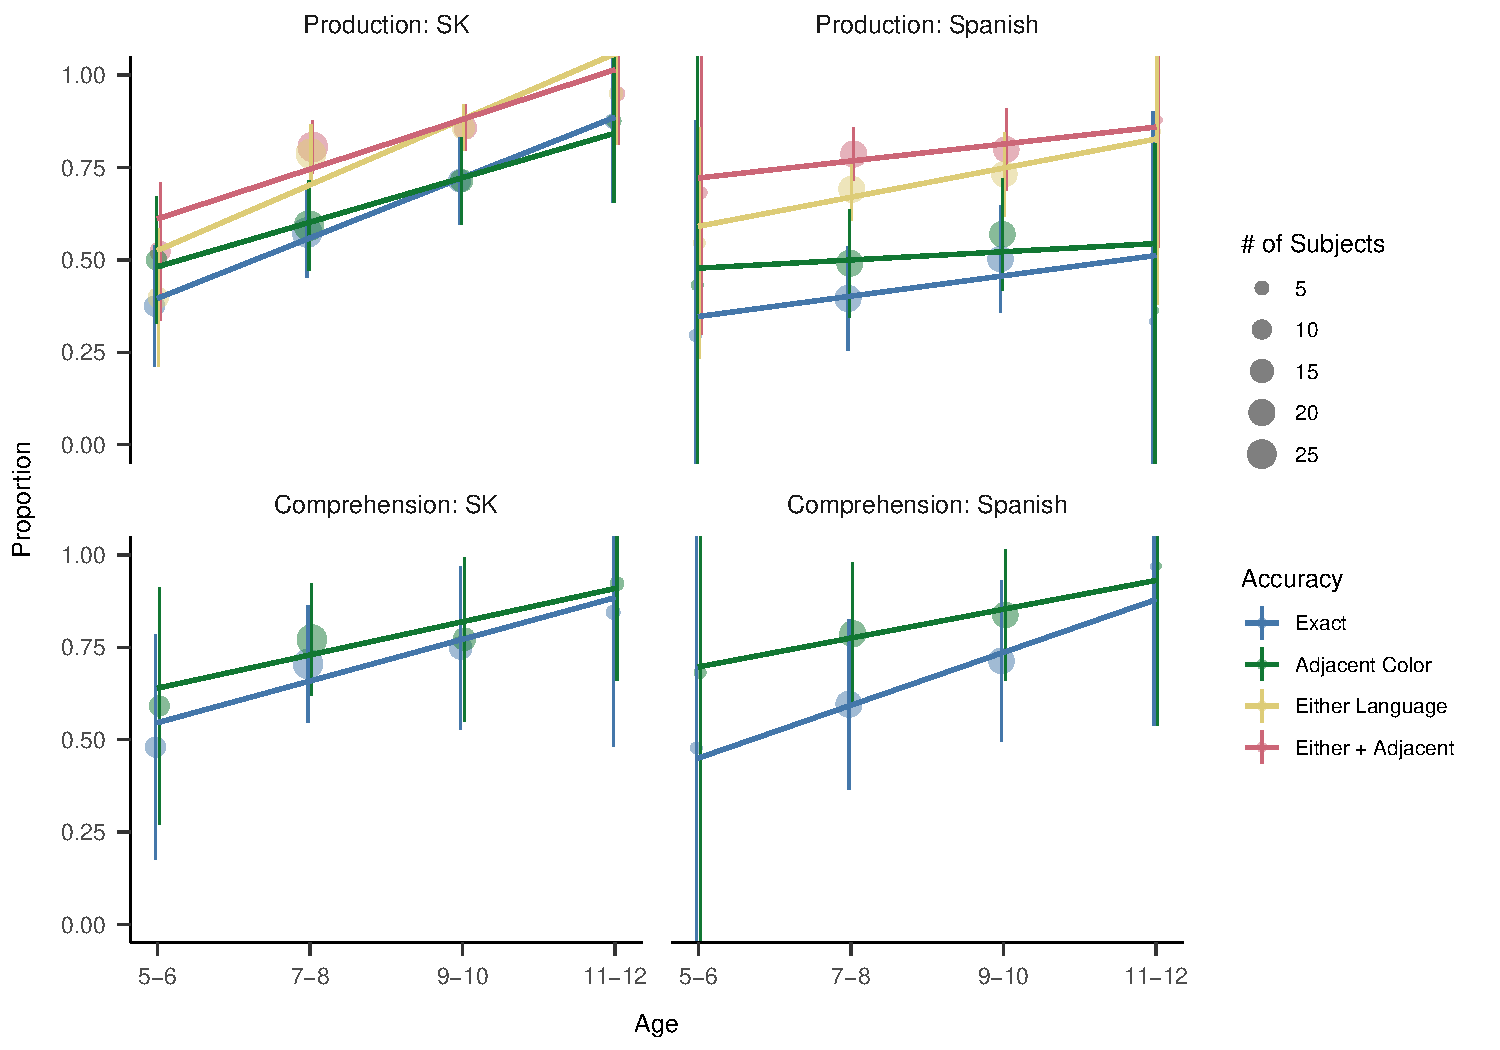
\includegraphics{amazon_color_files/figure-latex/study23-accuracy-1.pdf}
\caption{\label{fig:study23-accuracy}Proportion of accurate responses when applying different accuracy criteria, by age and study. Points show the mean for a 2-year age group (chosen arbitrarily for visualization) with 95\% confidence intervals. Lines show a linear fit, weighted by the number of datapoints in each age group.}
\end{figure}

\hypertarget{results-and-discussion-1}{%
\subsection{Results and Discussion}\label{results-and-discussion-1}}

We begin by presenting general results from both the production and comprehension tasks, and then turn to specific analyses of overextensions. Figure \ref{fig:study23-accuracy} shows general trends across measures. For Study 2, we saw robust developmental changes in both production and comprehension towards more adult-like performance. Because we had limited expectations regarding the amount of data that would be gathered during visits to the SK, we did not preregister our analyses. Thus all reported inferential statistics should be interpreted with some caution, and we do not adopt a specific cutoff of \(\alpha = .05\) for interpretation.

To quantify these trends, we fit generalized linear mixed-effects models (GLMMs) predicting accuracy for both production and comprehension tasks with fixed effects of age in years (centered), random slopes of age for each color, and random intercepts for each color and participant. When these models failed to converge, we removed random slopes. We found highly significant age effects for both production (\(\hat{\beta} = 0.85\), 95\% CI \([0.46, 1.24]\), \(z = 4.26\), \(p < .001\)) and comprehension (\(\hat{\beta} = 0.36\), 95\% CI \([0.18, 0.54]\), \(z = 3.85\), \(p < .001\)). Most children in our study knew some SK color words, but few except some of the oldest children knew all of them.

\begin{figure}
\centering
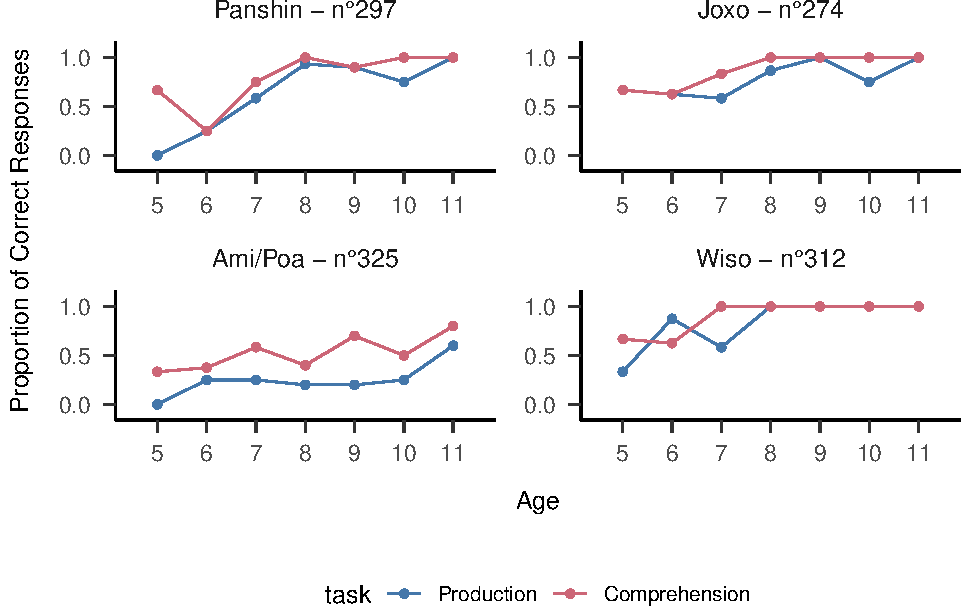
\includegraphics{amazon_color_files/figure-latex/study2-task-compare-plot-1.pdf}
\caption{\label{fig:study2-task-compare-plot}Production and comprehension data for selected color chips, plotted by age group.}
\end{figure}

\hypertarget{production-vs.-comprehension}{%
\subsubsection{Production vs.~comprehension}\label{production-vs.-comprehension}}

While overall, production and comprehension accuracies were quite close, there were exceptions. For some term-chip pairings such as ``ami/pua'' and ``pei/xo,'' children failed to produce the correct term in the production task but performed substantially better during the comprehension task (Figure \ref{fig:study2-task-compare-plot}). While there was a consistent ordering of tasks (production always first), there was no feedback on the production task, thus we think it is unlikely that children learned (or remembered) these labels as a function of task order. More likely is that these labels are relatively lower frequency and some children recognized them despite being unable to produce them.

\hypertarget{age-of-acquisition}{%
\subsubsection{Age of Acquisition}\label{age-of-acquisition}}

Following Frank et al. (2021), we used the dichotomous responses given during the production task to predict the ``age of acquisition'' when at least half of SK children are predicted to properly label a particular chip. First, we split responses by the prompted chip for which each participant had a single entry. For each chip, we attempted to fit a generalized linear model by robust methods (Maechler et al., 2020) with the structure \texttt{accuracy\ of\ response\ {[}0\ or\ 1{]}\ \textasciitilde{}\ age}. The coefficients for age ranged from 0.33 (odds of success multiplied by \(\exp{(\hat{\beta})}\) = 1.40 with every added year of age) to 1.35 (odds multiplied by \(\exp{(\hat{\beta})}\) = 3.80). To find age of acquisition, we then predicted the probability of success for the range of participant ages, 5.40- to 11.70-years-old at increments of 0.05 years, and selected the earliest age at which the accuracy crossed 0.5.

Using this method, we predict that half of SK children first learn to label the ``joxo'' chip (white) at 5.4 years of age. This is followed by the ``wiso'' chip (black) at 5.5, the ``hoshin'' chip (red) at 6.2, the ``panshin'' chip (yellow) at 7.2, the ``yankon'' chip (green) at 7.8, the ``nai'' chip (sky-blue; ``yankon'' also accepted) at 9.4, and the ``yankon''/``panshin'' chip (greenish-yellow) at 9.5. The model for one chip (``purple'') did not predict that age of acquisition would have been met within our age range, with an estimated probability of 46\% of children successfully labelling at 11.5 years of age.\footnote{It is worth noting that in Study 1, adult participants used 7 different labels for this chip (\emph{ambi}, \emph{ami}, \emph{jimi}, \emph{joshin}, \emph{kari}, \emph{morado}, and \emph{yankon}), none of which were used more than 25\% of the time.}

Our predictions suggest that SK children obtain color term knowledge at notably older ages compared to English-speaking children in the United States (Wagner et al., 2013). Further, the ordering of acquisition is substantially different from that attested in previous studies. It is an interesting question what properties of children's input or the color terms themselves lead to this order of acquisition. Following Yurovsky et al. (2015), we might speculate about the potential that ``joxo'' is substantially higher frequency in SK than ``white'' is in English.

\hypertarget{language-switching}{%
\subsubsection{Language switching}\label{language-switching}}

Over a quarter (27\%) of all responses were given in Spanish, despite children being prompted solely in SK (i.e., labeling a \emph{panshin}-colored chip as ``amarillo''). The distribution of Spanish responses was non-random, with median use in 2/8 trials (\emph{IQR} = 0-5). We did not find a significant correlation between age and number of trials with Spanish-language responses throughout the production task (\(t(55) = -0.97\), \(p = .335\)).

\begin{table}[tbp]

\begin{center}
\begin{threeparttable}

\caption{\label{tab:study1-entropy-table}Naming entropy by color chip and whether the chip was used in Study 2 and Study 3.}

\begin{tabular}{llllll}
\toprule
Chip ID & \multicolumn{1}{c}{Entropy} & \multicolumn{1}{c}{Study 2} & \multicolumn{1}{c}{Study 3} & \multicolumn{1}{c}{Shipibo term} & \multicolumn{1}{c}{Spanish term}\\
\midrule
1 & 0.71 & × &  & Nai & Celeste\\
46 & 1.72 &  & × & - & Gris\\
65 & 1.21 &  & × & - & Rosa\\
121 & 1.49 &  & × & - & Naranja\\
234 & 0.00 & × & × & Pei/Xo & Verde\\
245 & 0.21 & × & × & Joshin & Rojo\\
266 & 0.82 &  & × & - & Marron\\
274 & 0.33 & × & × & Joxo & Blanco\\
291 & 0.90 &  & × & - & Azul\\
297 & 0.21 & × & × & Panshin & Amarillo\\
312 & 0.80 & × & × & Wiso & Negro\\
320 & 1.34 & × &  & Barin Poi & Mierda sol\\
325 & 1.94 & × & × & Ami/Pua & Morado\\
\bottomrule
\end{tabular}

\end{threeparttable}
\end{center}

\end{table}

As a further exploratory analysis, we attempted to assess whether low naming consensus amongst adult SK speakers may be linked to children's naming strategies by quantifying naming entropy (following Gibson et al., 2017). We computed the naming entropy for each chip by computing the probabilities for each chip \(c\) to be named with a particular label \(l\) (\(p(l \mid c)\)) and then taking \(H(c) = -\sum_{l}{p(l\mid c) \log[p(l \mid c)]}\) (see entropy values by chip in Table \ref{tab:study1-entropy-table}).
To assess the hypothesis that naming entropy in adults was related to Spanish use in children, we fit a GLMM to predict likelihood of switching languages from SK to Spanish (a binary variable) as a function of child age, entropy of the chip's naming distribution for adults in Study 1, and their interaction (as well as random effects of subject). Despite age not being very correlated with overall frequency of Spanish responses, within this model, we found a trending but ultimately non-significant trend of older children being less likely to respond in Spanish (\(\hat{\beta} = -0.44\), 95\% CI \([-0.96, 0.07]\), \(z = -1.69\), \(p = .092\)). Children were significantly more likely to respond in Spanish when presented with a chip with greater entropy (low naming consensus) among adult participants in Study 1 (\(\hat{\beta} = 1.70\), 95\% CI \([1.15, 2.24]\), \(z = 6.10\), \(p < .001\)). We found a marginal, but non-significant positive interaction between age and entropy (\(\hat{\beta} = 0.30\), 95\% CI \([-0.03, 0.62]\), \(z = 1.78\), \(p = .074\)), suggesting greater Spanish use from older children for chips with low adult agreement. Together these findings suggest that children rely on language-switching to describe chips which lack consensus among adults.

\hypertarget{overextensions}{%
\subsubsection{Overextensions}\label{overextensions}}

One reason to use Spanish would be if children fail to recall the proper SK color term but do know the proper mapping in Spanish. But another possibility is that children may have more imprecise representations and choose to respond with a same-language but adjacent color term (i.e., labeling a \emph{panshin}-colored chip as ``joshin''). Following Wagner et al. (2013), we aggregated across color chips and examined the pattern of children's first responses, categorizing them as same-language, adjacent, and different-language. We used a GLMM to assess whether calculated word entropy and age were associated with frequency of adjacent responses. We predicted the outcome using fixed effects of age in years (centered) and entropy, with random effects of participant. We found that younger children were more likely to respond with SK-language adjacent terms (\(\hat{\beta} = -0.96\), 95\% CI \([-1.58, -0.34]\), \(z = -3.02\), \(p = .002\)) but chip entropy did not predict this strategy (\(\hat{\beta} = -1.38\), 95\% CI \([-3.06, 0.29]\), \(z = -1.62\), \(p = .106\)). Further, coefficients in this model were almost identical to the coefficient for strict scoring, confirming the impression that these overextensions were relatively rare compared to the use of Spanish terms.

\hypertarget{study-3}{%
\section{Study 3}\label{study-3}}

Noting the apparent strategy of language switching from SK to Spanish seen in Study 2, we designed Study 3 as its complement. Here, we tested children's production and comprehension of Spanish color terms with a similar protocol to Study 2 but with a different set of chips meant to represent the prototypical basic colors within the Spanish color system. Our goal was to more directly probe SK children's knowledge of the Spanish language and its color term lexicon as well as to observe whether children would employ language-switching as a strategy similar to what was seen in Study 2.

\hypertarget{methods-2}{%
\subsection{Methods}\label{methods-2}}

\hypertarget{participants-2}{%
\subsubsection{Participants}\label{participants-2}}

We recruited a separate sample of 46 children (16 boys) ages 5- to 11-years-old from the neighborhood of Bena Jema in Yarinacocha and from Bawanisho. Recruitment occurred either through interested parents or a local school. As in Study 2, we received consent from parents and, if in a school environment, teachers as well.

\hypertarget{materials-and-procedure-2}{%
\subsubsection{Materials and procedure}\label{materials-and-procedure-2}}

Based on Study 1, we selected 11 color chips to serve as prototypical instances of prominent Peruvian Spanish color terms. These color chips included 6 also used during Study 2: green (n°234), red (n°245), white (n°274), yellow (n°297), black (n°312) , and purple (n°325). Five additional chips were selected: gray (WCS n°46), pink (n°65), orange (n°121), brown (n°266), and blue (n°291) (see Appendix 1). The blue chips differed between Studies 2 and 3 as we decided that the prototypical hues for \emph{yankon} and \emph{azul} differed enough to warrant the use of a different chip.

As we found that many SK children in our sample were not very fluent in Spanish -- despite receiving some school instruction in Spanish -- the production and comprehension tasks were both conducted in SK, and Spanish was only used for color terms (i.e., Spanish color terms were embedded within otherwise SK sentences). In both tasks, a participant would sit at a table across from the experimenter with 11 color chips in front. As in Study 2, the production task was always performed prior to the comprehension task.

\hypertarget{production-task-1}{%
\subsection{Production task}\label{production-task-1}}

The procedure was similar to that of both Studies 1 and 2. The experimenter would introduce a participant to the general procedure and aims of the study. Despite much of the study being conducted in SK, the experimenter would specify that participants would be expected to provide color terms in Spanish. The experimenter would then ask: ``What is the color of this chip?'' If the participant responded in SK, the experimenter would record their response but further ask: ``What is the name of this color in Spanish?'' If a participant responded with ``I don't know'' to this prompt, the experimenter would not prompt any further and would move forward to the next chip. As a result, some responses lack Spanish-language basic level terms and only consist of non-basic and/or SK color terms. In total, we collected production data for 11 color chips. For each chip, the data include either one response (when children provided a Spanish basic color term in the first trial) or two to three responses (when children's initial responses were either non-basic and/or in SK).

\hypertarget{comprehension-task-1}{%
\subsubsection{Comprehension task}\label{comprehension-task-1}}

The procedure was similar to that of Study 2. The experimenter would ask: Can you give me the {[}\emph{color term}{]} chip? For 11 Spanish color terms. The choice of these terms was based on both previous studies examining Spanish color terms as well as responses given by adult participants in Study 1 (as some adult participants used Spanish color terms to label particular color chips). The 11 terms used as prompts were ``blanco'' (white), ``verde'' (green), ``rojo'' (red), ``amarillo'' (yellow), ``azul'' (blue), ``negro'' (``black''), ``naranja'' (orange), ``gris'' (gray), ``morado'' (purple), ``marrón'' (brown), and ``rosa'' (pink). Since each color term was best instantiated by a single color chip and lacked the ambiguity seen with certain SK color terms, we defined a correct response as choosing the single color chip that matched the word, in contrast to Study 2.

\hypertarget{results-and-discussion-2}{%
\subsection{Results and Discussion}\label{results-and-discussion-2}}

As in Study 2, we observed age-related changes in color term accuracy for both production and comprehension. Aggregate results are visualized in Figure \ref{fig:study23-accuracy}. To assess these, we again fit GLMMs for both production and comprehension tasks with an identical structure to Study 2. Age was a significant predictor of accuracy in the comprehension task (\(\hat{\beta} = 0.63\), 95\% CI \([0.21, 1.06]\), \(z = 2.90\), \(p = .004\)), but the age effect weakened in the production task (\(\hat{\beta} = 0.33\), 95\% CI \([-0.06, 0.72]\), \(z = 1.65\), \(p = .098\), see Figure \ref{fig:study23-accuracy}).

Like Study 2, over a quarter (30\%) of all responses were given in SK, despite being prompted to respond in Spanish. There was significant variation in language-switching with some children responding solely in Spanish while others responded in SK for upwards of 9/11 trials (\emph{Mdn} = 5 trials, \emph{IQR} = 1.25-6). We found only a marginal correlation between age and accuracy (\(t(44) = 1.91\), \(p = .063\)) and no significant correlation between age and language-switching (\(t(44) = 0.44\), \(p = .663\)).

To assess our hypothesis that older children would have more Spanish-language exposure and color term knowledge, we included age as a predictor in our GLMM assessing the effect of adult color naming entropy on likelihood to switch languages from Spanish to SK, similar to the one we fit for Study 2. This model did not show a significant interaction between age and adult color naming entropy (\(\hat{\beta} = -0.27\), 95\% CI \([-0.63, 0.09]\), \(z = -1.49\), \(p = .137\)), however one without the interaction term did show an entropy effect (\(\hat{\beta} = -1.49\), 95\% CI \([-2.07, -0.92]\), \(z = -5.10\), \(p < .001\)), tending to respond in SK for low-entropy items (those that were presumably more prototypical for the SK words). There was no significant effect of age (\(\hat{\beta} = -0.02\), 95\% CI \([-0.49, 0.45]\), \(z = -0.08\), \(p = .939\)). Across studies, it appears that children preferred to respond in SK when presented with a chip for which adults had high consensus about the SK label, and in Spanish for low-consensus chips.

Similar to Study 2, we adopted alternative scoring to accommodate language-switching from Spanish to SK (different-language) and adjacent same-language responses. We used a GLMM identical to that of Study 2 in order to assess whether changes in scoring criteria were associated with significant changes in task performance for production. Age was again a weaker predictor for production accuracy even with this more lenient scoring (\(\hat{\beta} = 0.25\), 95\% CI \([-0.07, 0.58]\), \(z = 1.53\), \(p = .126\)), in concordance with earlier analyses. However, we did find that participants had greater accuracy when we included SK responses (\(\hat{\beta} = 1.76\), 95\% CI \([1.43, 2.08]\), \(z = 10.46\), \(p < .001\)) or adjacent same-language responses (\(\hat{\beta} = 0.51\), 95\% CI \([0.20, 0.81]\), \(z = 3.27\), \(p = .001\)). In sum, we find frequent use of language switching in both Studies 2 and 3, but only Study 3 exhibits significant use of same-language but adjacent terms.

We speculate that early, informal Spanish language exposure can explain the discrepancies seen in Studies 2 and 3. With limited knowledge of Spanish color terms, children may spontaneously supplement their color term knowledge with Spanish terms during SK-language Study 2 but struggle to succeed in a more systematic evaluation in Study 3. More generally, we see children relying on a mixture of strategies to communicate colors even in the absence of mastery in either language.

\hypertarget{general-discussion}{%
\section{General Discussion}\label{general-discussion}}

In three studies, we mapped the color vocabulary of the Shipibo-Konibo (SK) language and used these data to study the development of color vocabulary in SK children growing up in a bilingual environment. This effort fills a gap in studies of color word development in non-WEIRD cultures and more generally parallels other efforts to use methods from language development to study populations that are under-represented in developmental science (Fortier et al., under review; e.g., Piantadosi et al., 2014).

With respect to the adult data, we found that the SK color vocabulary was relatively unchanged over the generations since the original WCS. Several interesting observations emerged, however. First, consistent with our review of the prior literature, there was substantial use of non-basic color terms (including both ad hoc and luminance-based terms). These terms were used more often in SK than in Spanish, supporting the idea that Amazonian languages may make greater use of ad hoc color terms (at least in naming tasks) than Spanish (Everett, 2005). Our data do not speak to whether this use is due to a desire to succeed on specific experimental tasks or whether it is comparable to use in naturalistic contexts. Nevertheless our findings are reminiscent of a suggestion by Levinson (2000) that even purported basic level terms in Yélî Dnye did not fully span hue space and were often supplemented creatively with ad hoc terms.

Second, we saw substantial use of Spanish terms by adults, even though the task was conducted in SK. We speculate that this is because the adults were recognizing focal colors for Spanish basic level terms that have no parallel in SK (e.g., ``morado'' for purple). On the other hand, ``naranja'' could in fact be a loan word that has been assimilated into the SK vocabulary by some speakers. Either way, this finding suggests an adaptive use of color vocabulary from both languages to succeed on the labeling task; future work will be required to understand whether such strategies are used in naturalistic communication as well.

When we turned to the children's data, we observed a much longer developmental trajectory for color word learning than is observed in contemporary English-learning children within the United States. As noted by Bornstein (1985), however, it is a very recent development that color terms are mastered as early as they are -- one hundred years ago, English-speaking US children's timeline of acquisition looked broadly similar to that observed in our study for SK children. We can only speculate as to the drivers of this historical change, but the industrialization hypothesis propounded by Gibson et al. (2017) appears to be a reasonable starting point. That is, industrialization allows for the production of identical objects that are usefully distinguished by color labeling. This communicative pressure can then lead to differentiation of color terms on a historical timescale and -- relevant to our study here -- is a likely driver of faster acquisition of color words by children.\footnote{These speculations are informed by personal experience; the children of one author both learned their color terms in their second years of life through repeated practice with sets of manufactured plastic artifacts that varied only in hue, providing ideal teaching examples.} SK children have some access to such artifacts, but according to anthropological accounts it is substantially sparser.

We did not find strong evidence for overextension in children's SK production or comprehension (with one or two exceptions), though there was somewhat more evidence for overextension in Spanish. This asymmetry might be due to less systematic or consistent exposure to Spanish vocabulary, but this explanation is merely speculative. We did, however, observe robust evidence for mixing and competition between the SK and Spanish color systems. Children differentially used Spanish terms in Study 2 when there was high uncertainty about the SK label for a particular color chip among adults in Study 1. Similarly, they reached into their SK vocabulary in Study 3 when there was high consistency in SK labels among adults. These findings suggest that children were using their bilingual vocabulary adaptively to choose terms that are more likely to be interpreted correctly. Further, they suggest a potential route for functionally-driven language change, such that Spanish terms are borrowed -- and perhaps eventually conventionalized -- by children in cases where adult input indicates uncertainty about the appropriate SK label.

Comprehension is thought to proceed production in language development generally (Clark, 2009; Frank et al., 2021) and in color word learning specifically (Wagner et al., 2018). In our data we did not observe large asymmetries between comprehension and production. Yet this result comes with caveats. First, comprehension and production tasks are by their nature different and have different demands (Sandhofer \& Smith, 1999); this was especially true in our case given that the two tasks were sequenced and scored somewhat differently. Thus, we have chosen not to make quantitative comparisons between accuracies across these two tasks. Second, production and comprehension may be especially divergent for the youngest children, those who have the most difficulty with phonological encoding and the motoric aspects of production (Frank et al., 2021); there is less evidence for production-comprehension divides in middle childhood. One natural question is whether comprehension and production dissociated in earlier times when US English-learners similarly acquired colors late; unfortunately we do not know of data that could be used to evaluate this question.

Our data here are consistent with models of color word meaning in which color word use is driven by functional need and languages adapt by developing vocabularies that appropriately allow for communication about those needs (Gibson et al., 2017; Zaslavsky et al., 2018). These models have not yet been generalized to either the bilingual setting or the acquisition setting, however. Our data suggest that functional language use can cross language boundaries, inviting models that consider code switching and borrowing as part of the process of change (e.g., Myslin \& Levy, 2015).

Studying SK children's learning provides a descriptive comparison to studies of color naming in children learning English in the US (the focus of the majority of developmental work). Nonetheless, it has a number of limitations, some shared with this previous literature and some due to the specifics of our study and context. First, we regrettably do not have access to the kind of deep ethnographic observations that would allow us to hazard generalizations about how color terms are used in daily life among the SK communities we studied. Second, our study of development is cross-sectional and does not afford precision regarding the specific knowledge state of individual children due to the limited length of the task. Third, the limited number of color chips that we investigated means that our ability to generalize about the precision of particular color generalizations is much more limited for the children than the adults (limiting our entropy analyses). Finally, and perhaps most prominently, the kinds of tasks that we used are likely more unfamiliar to all of our participants and especially our child participants than they are to the populations being tested in investigations of WEIRD cultures (e.g., US English-learning children). While the performance of the oldest children in our studies was close to ceiling, the lower performance observed with younger children could be in part a product of task unfamiliarity or other factors.

Going beyond convenience populations in experimental research with children is a new frontier for developmental science (Nielsen et al., 2017). Our work here suggests some of the benefits and challenges of this approach. On the positive, we can compare and generalize models of acquisition that are largely based on a single language and population (US English-acquiring children). At the same time, there is a paucity of resources describing language use, home environment, and cultural practices once we venture outside of WEIRD contexts. To best understand acquisition across cultures, we must document both children's knowledge and the structure of their environments.

\newpage

\hypertarget{references}{%
\section{References}\label{references}}

\begingroup
\setlength{\parindent}{-0.5in}
\setlength{\leftskip}{0.5in}

\hypertarget{refs}{}
\begin{CSLReferences}{1}{0}
\leavevmode\hypertarget{ref-aragon2016}{}%
Aragón, K. (2016). \emph{Color language and color categorization} (G. Paulsen, M. Uusküla, \& J. Brindle, Eds.). Cambridge Scholars.

\leavevmode\hypertarget{ref-bartlett1977}{}%
Bartlett, E. J. (1977). \emph{Semantic organization and reference: Acquisition of two aspects of the meaning of color terms}. Biennial Meeting of the Society for Research in Child Development.

\leavevmode\hypertarget{ref-berlin1969}{}%
Berlin, B., \& Kay, P. (1969). \emph{Basic color terms: Their universality and evolution}. University of California Press.

\leavevmode\hypertarget{ref-bornstein1985}{}%
Bornstein, M. H. (1985). On the development of color naming in young children: Data and theory. \emph{Brain and Language}, \emph{26}(1), 72--93.

\leavevmode\hypertarget{ref-bornstein2015}{}%
Bornstein, M. H. (2015). Emergence and early development of color vision and color perception. In \emph{Handbook of {C}olor {P}sychology}. Cambridge University Press.

\leavevmode\hypertarget{ref-bornstein1976}{}%
Bornstein, M. H., Kessen, W., \& Weiskopf, S. (1976). Color vision and hue categorization in young human infants. \emph{Journal of Experimental Psychology: Human Perception and Performance}, \emph{2}(1), 115--129.

\leavevmode\hypertarget{ref-chater2010}{}%
Chater, N., \& Christiansen, M. H. (2010). Language acquisition meets language evolution. \emph{Cognitive Science}, \emph{34}(7), 1131--1157.

\leavevmode\hypertarget{ref-clark1973}{}%
Clark, E. V. (1973). \emph{Cognitive development and acquisition of language} (pp. 65--110). Academic Press.

\leavevmode\hypertarget{ref-clark1987}{}%
Clark, E. V. (1987). \emph{Mechanisms of language acquisition} (B. MacWhinney, Ed.; pp. 1--33). Psychology Press.

\leavevmode\hypertarget{ref-clark2009}{}%
Clark, E. V. (2009). \emph{First language acquisition}. Cambridge University Press.

\leavevmode\hypertarget{ref-culbertson2012}{}%
Culbertson, J., Smolensky, P., \& Legendre, G. (2012). Learning biases predict a word order universal. \emph{Cognition}, \emph{122}(3), 306--329.

\leavevmode\hypertarget{ref-everett2005}{}%
Everett, D. L. (2005). Cultural constraints on grammar and cognition in pirah{ã} another look at the design features of human language. \emph{Current Anthropology}, \emph{46}(4), 621--646.

\leavevmode\hypertarget{ref-forbes2019}{}%
Forbes, S. H., \& Plunkett, K. (2019). Infants show early comprehension of basic color words. \emph{Developmental Psychology}, \emph{55}(2), 240.

\leavevmode\hypertarget{ref-forbes2020}{}%
Forbes, S. H., \& Plunkett, K. (2020). Linguistic and cultural variation in early color word learning. \emph{Child Development}, \emph{91}(1), 28--42.

\leavevmode\hypertarget{ref-fortierunderreview}{}%
Fortier, M., Kellier, D., Fernández Flecha, M., \& Frank, M. C. (under review). \emph{Ad-hoc pragmatic implicatures among {S}hipibo-{K}onibo children in the {P}eruvian {A}mazon}.

\leavevmode\hypertarget{ref-frank2020}{}%
Frank, M. C., Braginsky, M., Yurovsky, D., \& Marchman, V. A. (2021). \emph{Variability and consistency in early language learning: The wordbank project}. MIT Press.

\leavevmode\hypertarget{ref-frank2014}{}%
Frank, M. C., \& Goodman, N. D. (2014). Inferring word meanings by assuming that speakers are informative. \emph{Cognitive Psychology}, \emph{75}, 80--96.

\leavevmode\hypertarget{ref-franklin2005}{}%
Franklin, A., Pilling, M., \& Davies, I. (2005). The nature of infant color categorization: Evidence from eye movements on a target detection task. \emph{Journal of Experimental Child Psychology}, \emph{91}(3), 227--248.

\leavevmode\hypertarget{ref-gibson2017}{}%
Gibson, E., Futrell, R., Jara-Ettinger, J., Mahowald, K., Bergen, L., Ratnasingam, S., Gibson, M., Piantadosi, S. T., \& Conway, B. (2017). Color naming across languages reflects color use. \emph{Proceedings of the National Academy of Sciences}, \emph{114}(40), 10785--10790.

\leavevmode\hypertarget{ref-henrich2010}{}%
Henrich, J., Heine, S. J., \& Norenzayan, A. (2010). The weirdest people in the world? \emph{Behavioral and Brain Sciences}, \emph{33}(2-3), 61--83.

\leavevmode\hypertarget{ref-berlin2009}{}%
Kay, P., Berlin, B., Maffin, L., Merrifield, W. R., \& Cook, R. (2009). \emph{The world color survey}. Center for the Study of Language; Information.

\leavevmode\hypertarget{ref-kristol1980}{}%
Kristol, A. M. (1980). Color systems in southern italy: A case of regression. \emph{Language}, \emph{56}(1), 137--145.

\leavevmode\hypertarget{ref-lathrap1970}{}%
Lathrap, D. W. (1970). \emph{The {U}pper {A}mazon}. Thames; Hudson.

\leavevmode\hypertarget{ref-levinson2000}{}%
Levinson, S. C. (2000). Yélî dnye and the theory of basic color terms. \emph{Journal of Linguistic Anthropology}, \emph{10}(1), 3--55.

\leavevmode\hypertarget{ref-lillo2018}{}%
Lillo, J., González-Perilli, F., Prado-León, L., Melnikova, A., Álvaro, L., Collado, J. A., \& Moreira, H. (2018). Basic color terms (BCTs) and categories (BCCs) in three dialects of the {S}panish language: Interaction between cultural and universal factors. \emph{Frontiers in Psychology}, \emph{9}.

\leavevmode\hypertarget{ref-R-robustbase}{}%
Maechler, M., Rousseeuw, P., Croux, C., Todorov, V., Ruckstuhl, A., Salibian-Barrera, M., Verbeke, T., Koller, M., Conceicao, E. L. T., \& Anna di Palma, M. (2020). \emph{Robustbase: Basic robust statistics} (R package version 0.93-6).

\leavevmode\hypertarget{ref-monroy1989}{}%
Monroy, M., \& Custodio, S. (1989). Algunos usos de los t{é}rminos del color en el espa{ñ}ol de {C}olombia {[}some uses of color terms in {C}olombian {S}panish{]}. \emph{Thesaurus: Bolet{í}n Del Instituto Caro y Cuervo}, \emph{44}(2), 441--450.

\leavevmode\hypertarget{ref-morin1973}{}%
Morin, E. (1973). \emph{Le paradigme perdu: La nature humaine {[}the lost paradigm: The human nature{]}}. {É}ditions du Seuil.

\leavevmode\hypertarget{ref-Myers1974}{}%
Myers, T. P. (1974). {S}panish contacts and social change on the {U}cayali {R}iver, {P}eru. \emph{Ethnohistory}, \emph{21}(2), 135--137.

\leavevmode\hypertarget{ref-myslin2015}{}%
Myslin, M., \& Levy, R. (2015). Code-switching and predictability of meaning in discourse. \emph{Language}, \emph{91}(4), 871--905.

\leavevmode\hypertarget{ref-nielson2017}{}%
Nielsen, M., Haun, D., Kärtner, J., \& Legare, C. H. (2017). The persistent sampling bias in developmental psychology: A call to action. \emph{Journal of Experimental Child Psychology}, \emph{162}, 31--38.

\leavevmode\hypertarget{ref-piantadosi2014}{}%
Piantadosi, S. T., Jara‐Ettinger, J., \& Gibson, E. (2014). Children's learning of number words in an indigenous farming‐foraging group. \emph{Developmental Science}, \emph{17}(4), 553--563.

\leavevmode\hypertarget{ref-regier2007}{}%
Regier, T., Kay, P., \& Khetarpal, N. (2007). Color naming reflects optimal partitions of color space. \emph{Proceedings of the National Academy of Sciences}, \emph{104}(4), 1436--1441.

\leavevmode\hypertarget{ref-saji2015}{}%
Saji, N., Asano, M., Oishi, M., \& Imai, M. (2015). How do children construct the color lexicon?: Restructuring the domain as a connected system. \emph{CogSci}.

\leavevmode\hypertarget{ref-sandhofer1999}{}%
Sandhofer, C. M., \& Smith, L. B. (1999). Learning color words involves learning a system of mappings. \emph{Developmental Psychology}, \emph{35}(3), 668--679.

\leavevmode\hypertarget{ref-sedivy2003}{}%
Sedivy, J. C. (2003). Pragmatic versus form-based accounts of referential contrast: Evidence for effects of informativity expectations. \emph{Journal of Psycholinguistic Research}, \emph{32}(1), 3--23.

\leavevmode\hypertarget{ref-stclair2016}{}%
St. Clair, K. (2016). \emph{The secret lives of colour}. John Murray.

\leavevmode\hypertarget{ref-surralles2016}{}%
Surrallés, A. (2016). On contrastive perception and ineffability: Assessing sensory experience without colour terms in an amazonian society. \emph{Journal of the Royal Anthropological Institute}, \emph{22}(4), 962--979.

\leavevmode\hypertarget{ref-tournon2002}{}%
Tournon, J. (2002). \emph{La merma m{á}gica: Vida e historia de los {S}hipibo-{C}onibo del {U}cayali {[}the magic reduction: Life and history of the {U}cayali {S}hipibo-{C}onibo{]}}. Centro Amaz{ó}nico de Antropolog{í}a y Aplicaci{ó}n.

\leavevmode\hypertarget{ref-wagner2013}{}%
Wagner, K., Dobkins, K., \& Barner, D. (2013). Slow mapping: Color word learning as a gradual inductive process. \emph{Cognition}, \emph{127}, 307--317.

\leavevmode\hypertarget{ref-wagner2018}{}%
Wagner, K., Jergens, J., \& Barner, D. (2018). Partial color word comprehension precedes production. \emph{Language Learning and Development}, \emph{14}(4), 241--261.

\leavevmode\hypertarget{ref-yurovsky2015}{}%
Yurovsky, D., Wagner, K., Barner, D., \& Frank, M. C. (2015). Signatures of domain-general categorization mechanisms in color word learning. \emph{Proceedings of the 37th Annual Conference of the Cognitive Science Society}.

\leavevmode\hypertarget{ref-zaslavsky2018}{}%
Zaslavsky, N., Kemp, C., Tishby, N., \& Regier, T. (2018). \emph{Color naming reflects both perceptual structure and communicative need} (Vols. 1250--1255). Proceedings of the 40th Annual Conference of the Cognitive Science Society.

\end{CSLReferences}

\endgroup


\end{document}
